% PromptShift v3 report. On Overleaf: open the official ACL template, replace its
% main.tex with this file, and upload references.bib and the figures/ folder.
% Locally, acl_preview.sty stands in for acl.sty.
\documentclass[11pt]{article}
\IfFileExists{acl.sty}{\usepackage[final]{acl}}{\usepackage{acl_preview}}
\usepackage{times}
\usepackage{latexsym}
\usepackage[T1]{fontenc}
\usepackage[utf8]{inputenc}
\usepackage{microtype}
\usepackage{graphicx}
\usepackage{booktabs}
\usepackage{array}
\usepackage{amsmath}
\usepackage{amssymb}
\usepackage{textcomp}

\title{Same Post, Different Prompt: Is LLM Prompt Sensitivity in\\Offensive-Language Annotation an Artefact of Memorised Data?}

\author{Raywin Cruz Thumma Rayappan \quad Namrath Basavaraju \quad Jagadeesh Gunti \\
  Joseph Velangini Pravallika Are \quad Erhisohwode Assurance Ovie \\
  University of Mannheim \\
  IS 617 Large Language Models for the Economic and Social Sciences, HWS 2026}

\begin{document}
\maketitle

\begin{abstract}
Social scientists increasingly use large language models (LLMs) as annotators, yet the labels they produce depend on how the instruction is worded and on whether a codebook definition is given. Benchmark datasets such as OLID (2019) are probably part of the models' training data, so prompt-sensitivity estimates obtained on them might reflect memorisation. We compare three open-weight LLMs (Gemma~4, Qwen~3.6, Llama~3.3) under eight prompt conditions (three one-sentence wordings, each with and without OLID's definition, plus two exact repeats) on the OLID test set (860 posts) and on 400 Bluesky posts written after all three models were released, which we labelled ourselves. Hypotheses and analyses were frozen before the models saw the new posts. Wording changed about 3\% of labels on both datasets, and the difference between datasets was not significant for any model. Adding the definition reduced the error in the estimated share of offensive posts for all three models (e.g.\ Gemma: 13.2 to 4.2 percentage points). Accuracy could not be compared across datasets because our labels agreed only moderately with OLID's ($\kappa \le 0.43$). Five contamination probes, each run on the new posts as a negative control, found no sign that OLID is memorised.
\end{abstract}

\section{Introduction}

LLMs are now routinely used to label text in computational social science (CSS), for example to estimate how much offensive language circulates on a platform. Several studies show that such labels are sensitive to the prompt: small rewordings and repeated identical requests change annotations \citep{reiss2023testing}, prompt format alone shifts accuracy \citep{sclar2024quantifying,mizrahi2024state}, and adding a definition changes the distribution of labels in CSS tasks including toxicity \citep{atreja2025prompt}.

Most of this evidence comes from public benchmarks. Benchmarks released before a model's training cut-off may be part of its training data \citep{golchin2024time}, and models perform better on datasets released before their cut-off than after it \citep{li2024task}. If a model has memorised a benchmark post, its answer may be anchored to what it has seen, and prompt sensitivity measured on that benchmark may not describe the model's behaviour on the new data a social scientist actually wants to label.

We test this directly with a temporal hold-out. We repeat a prompt-sensitivity design on the OLID test set \citep{zampieri-etal-2019-predicting,barbieri-etal-2020-tweeteval}, collected in 2019, and on posts written after all three models were publicly released, which therefore cannot be in their training data. Our research question is: \emph{do prompt wording and a codebook definition affect LLM annotation of offensive language differently on data the models have likely seen than on posts written after their release, and what are the consequences for prevalence estimates?}

Our contributions are: (1) a pre-specified comparison of wording sensitivity on likely-seen versus guaranteed-unseen data, with exact repeats as a chance baseline on both; (2) prevalence error, the quantity CSS studies usually report, as an outcome alongside F1; (3) a contamination battery in which every probe is also run on the unseen posts, so that we can see whether a probe can detect anything at all; and (4) a new, human-labelled set of 400 post-release posts collected with OLID's own sampling keywords.

\section{Related Work}

\paragraph{Prompt sensitivity in annotation.} \citet{reiss2023testing} shows that minor wording changes and repeated inputs lower ChatGPT's reliability. \citet{atreja2025prompt} vary definition inclusion, output type, explanation and length across four CSS tasks and find that prompt design changes both compliance and label distributions. \citet{errica-etal-2025-wrong} propose sensitivity (label change across rephrasings, without gold labels) and consistency metrics; our wording-disagreement measure follows the sensitivity idea. Because the effect of adding a definition is already known, we do not claim it as a finding; we test whether it holds on unseen data and what it does to prevalence.

\paragraph{Contamination.} Comparisons before and after a training cut-off are an established contamination signal \citep{li2024task}, but performance decay after the cut-off is not a clean signal \citep{zhang-etal-2026-test}. Instance-level probes include guided completion \citep{golchin2024time}, the Data Contamination Quiz \citep{golchin2025dcq} and Min-K\% Prob \citep{shi2024detecting}; membership inference on LLMs is often barely better than chance and confounded by time \citep{duan2024membership}. Closest to our work, \citet{casanova2026limits} find across nine LLMs and five toxicity datasets that performance tracks the fit between the model's concept and the dataset's definition rather than memorisation metrics. We differ in using data that cannot have been memorised and in studying prompt sensitivity and prevalence rather than accuracy alone.

\section{Data}

\paragraph{OLID.} We use the TweetEval offensive test split (OLID level A), pinned to revision \texttt{b3a375b}: 860 posts, of which 240 (27.9\%) are labelled offensive.

\paragraph{New posts.} We collected public posts from Bluesky, a Twitter-like platform, through its official search API, using the OLID sampling keywords that exist on Bluesky (\emph{you are, she is, he is, gun control, conservatives, antifa, MAGA, liberals}), month by month from 1 May to 15 November 2026. Llama~3.3 was released on 6 December 2024 with training data up to December 2023 \citep{meta2024llama33}; Gemma~4 was released on 2 April 2026 with data up to January 2025 \citep{gemma2026gemma4}; Qwen~3.6 was released in April 2026 \citep{qwen2026qwen36}. Every new post was therefore written after all three releases, and the collector rejects any post created before 1 May 2026 (31 posts fell outside the collection window). Of 15,561 returned posts, 11,405 remained after keeping English, original posts (no quote posts) with the keyword in the text and at least three content words, and 10,926 after removing exact and near duplicates (Jaccard $\geq 0.8$). We drew a stratified sample of 470 posts (58--59 per keyword, 64--72 per month, at most two per author) and split it into 400 main, 40 pilot and 30 calibration posts. As in OLID, mentions were replaced by \texttt{@USER} and links by \texttt{URL}. Counts and SHA-256 hashes of every file are stored in the repository.

\paragraph{Human labels.} An LLM cannot provide the gold labels without making the evaluation circular, so the team labelled the posts. The one-page guide reproduces OLID's level-A definitions verbatim with six invented examples. Two team members first labelled and discussed the 30 calibration posts, then labelled the 400 main posts and 100 OLID test posts mixed in as anchors, in separate random orders. A third team member labelled the 35 posts on which the two disagreed, and the final label is the majority. Agreement between the two annotators was good (Krippendorff's $\alpha = 0.78$, raw agreement 91.2\%; \citealp{krippendorff2018content}); 24.5\% of the 400 posts are offensive. Agreement with OLID's labels on the anchors was moderate (accuracy 0.78 and 0.77, Cohen's $\kappa = 0.43$ and $0.37$). The two annotators' offensive shares on the new posts differed (30.8\% vs.\ 22.5\%), so we also report all tests with annotator A's labels alone.

\section{Method}

\paragraph{Models and prompts.} We queried \texttt{gemma4-26b}, \texttt{qwen3.6-36b} and \texttt{llama-3.3-70b} through the University of Mannheim's maKI API (OpenAI-compatible), with temperature 0, at most 16 output tokens and first-token log probabilities recorded. Eight conditions cross three wordings (W0--W2), which differ only in the first sentence, with the presence of OLID's definition (D0--D2); R0 and RD0 repeat W0 and D0 exactly (Appendix~\ref{app:prompts}). Requests were sent in a seeded random order in which a repeat never directly follows its original, and every response was checked against the requested model name. This gives 20,640 calls on OLID and 9,600 on the new posts; one Llama answer on the new posts could not be parsed and is excluded from the affected estimands.

\paragraph{Hypotheses.} Each hypothesis is tested per model, one-sided, with a smallest effect size of interest (SESOI).
\textbf{H1}: excess wording sensitivity is higher on the new posts. Per post, excess sensitivity is the mean pairwise disagreement among W0--W2 minus $\mathbb{1}[\mathrm{W0} \neq \mathrm{R0}]$; $\Delta_1 = \mathrm{EWS}_{\text{new}} - \mathrm{EWS}_{\text{OLID}}$; SESOI 0.01.
\textbf{H2}: labelling quality is lower on the new posts: $\Delta_2$ is the difference in macro-F1, averaged over W0--W2 and D0--D2; SESOI 0.03.
\textbf{H3}: on the new posts, the definition reduces prevalence error. With $\mathrm{PE}_X$ the mean over the three wordings of $|\hat{p} - p_{\text{gold}}|$, the absolute difference between the predicted and the human offensive share, $\Delta_3 = \mathrm{PE}_D - \mathrm{PE}_W$; SESOI 0.02.

\paragraph{Inference.} We use percentile bootstrap with 10,000 resamples: independent resampling of posts within each dataset for H1 and H2 (class-stratified for H2) and paired, class-stratified resampling for H3. The nine primary tests are corrected with Holm's method \citep{holm1979simple} at $\alpha = 0.05$. Size is judged separately from significance: an effect is ``material'' if the 95\% bound clears the SESOI and ``practically equivalent'' if the interval lies within $\pm$SESOI; otherwise its size is inconclusive. We fixed in advance that H2 is not interpretable as a contamination effect if either annotator's $\kappa$ against OLID on the anchors falls below 0.60, because the two gold standards would then differ too much. The plan was committed to git before any model saw the new posts, and later changes are listed with reasons in a deviation log.

\paragraph{Contamination battery.} Each probe was run on 200 OLID training posts, 200 OLID test posts and the new posts that meet the probe's length rule: P1 guided minus general completion \citep[ROUGE-L;][]{golchin2024time}; P2 manual review of near-verbatim completions (ROUGE-L $\geq 0.7$); P3 accuracy gain when the prompt says the post is from OLID; P4 Min-K\% Prob ($k = 20\%$), with models excluded if more than 10\% of items fail; and P5 the Data Contamination Quiz, picking the original among three paraphrases. A probe counts as evidence only if OLID scores higher than the new posts.

\section{Results}

\begin{figure*}[t]
  \centering
  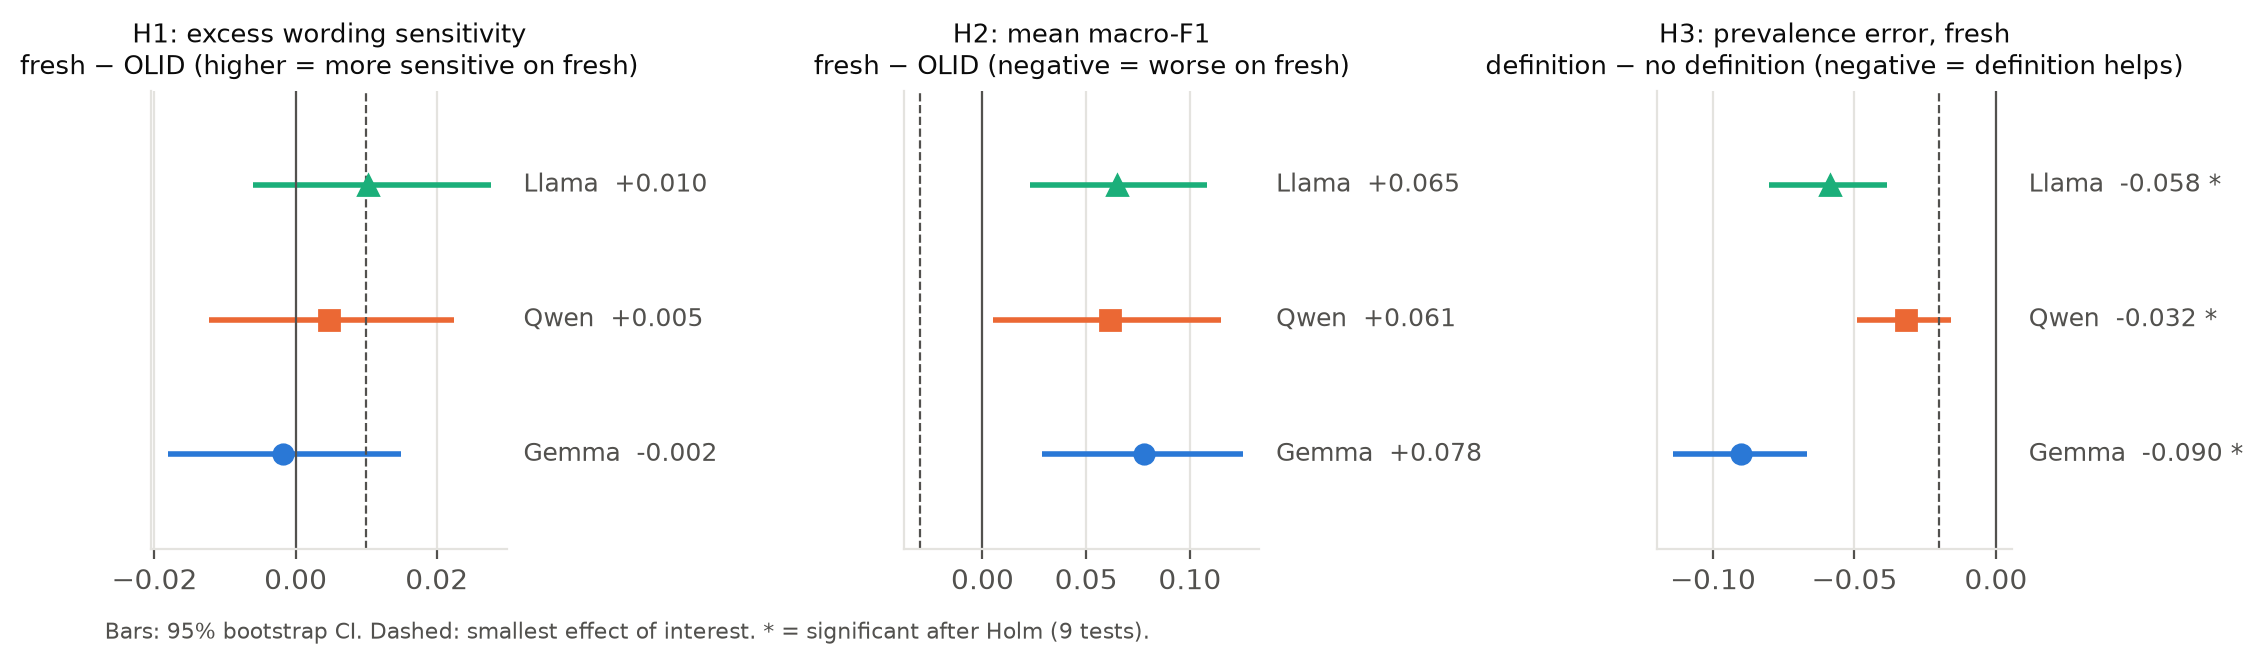
\includegraphics[width=\textwidth]{figures/fig5_v3_primary_tests.png}
  \caption{Primary tests. Points are estimates, bars 95\% bootstrap CIs, dashed lines the smallest effect of interest; * significant after Holm correction across nine tests.}
  \label{fig:primary}
\end{figure*}

\begin{table}[t]
  \centering\small
  \begin{tabular}{llrcr}
    \toprule
     & Model & $\Delta$ & 95\% CI & $p_{\text{Holm}}$ \\
    \midrule
    H1 & Gemma & $-0.002$ & [$-0.018$, $0.015$] & 1.000 \\
       & Qwen  & $0.005$ & [$-0.012$, $0.022$] & 1.000 \\
       & Llama & $0.010$ & [$-0.006$, $0.028$] & 0.687 \\
    \midrule
    H2 & Gemma & $0.078$ & [$0.029$, $0.126$] & 1.000 \\
       & Qwen  & $0.061$ & [$0.005$, $0.115$] & 1.000 \\
       & Llama & $0.065$ & [$0.023$, $0.108$] & 1.000 \\
    \midrule
    H3 & Gemma & $-0.090$ & [$-0.114$, $-0.067$] & 0.001 \\
       & Qwen  & $-0.032$ & [$-0.049$, $-0.016$] & 0.001 \\
       & Llama & $-0.058$ & [$-0.080$, $-0.038$] & 0.001 \\
    \bottomrule
  \end{tabular}
  \caption{Primary tests (new posts $n = 400$, OLID $n = 860$). H1 and H2: new minus OLID; H3: with minus without definition, on new posts. H2 is not interpretable (gold-label rule not met).}
  \label{tab:primary}
\end{table}

\paragraph{H1: wording sensitivity does not grow on unseen posts.} Changing one sentence of the instruction changed 2.5--3.0\% of labels per pair of wordings on OLID and 2.7--3.5\% on the new posts, while exact repeats changed 0--0.75\%. The dataset difference in excess sensitivity was small and not significant for any model (Table~\ref{tab:primary}, Figure~\ref{fig:primary}); its size is inconclusive, since the intervals include both zero and the SESOI. H1 is not supported.

\paragraph{H2: not interpretable.} Macro-F1 was higher on the new posts for every model (Gemma 0.81 vs.\ 0.73, Qwen 0.79 vs.\ 0.73, Llama 0.85 vs.\ 0.79), opposite to H2. Because both annotators' $\kappa$ against OLID was below the pre-set 0.60, we do not interpret this difference: it may reflect differences between the two gold standards rather than the models.

\paragraph{H3: the definition reduces prevalence error.} Without the definition, Gemma and Qwen labelled too few new posts offensive (11.3\% and 13.0\%) and Llama too many (35.3\%), against a human share of 24.5\%. With the definition, all three moved toward the human share (20.3\%, 16.2\%, 29.4\%; Figure~\ref{fig:prev}). Prevalence error fell from 13.2 to 4.2 percentage points for Gemma, 11.5 to 8.3 for Qwen and 10.8 to 4.9 for Llama; all three reductions are significant, material for Gemma and Llama and inconclusive in size for Qwen. OLID showed the same direction (descriptive, observed before the plan was frozen: $-0.085$, $-0.039$, $-0.040$).

\begin{figure*}[t]
  \centering
  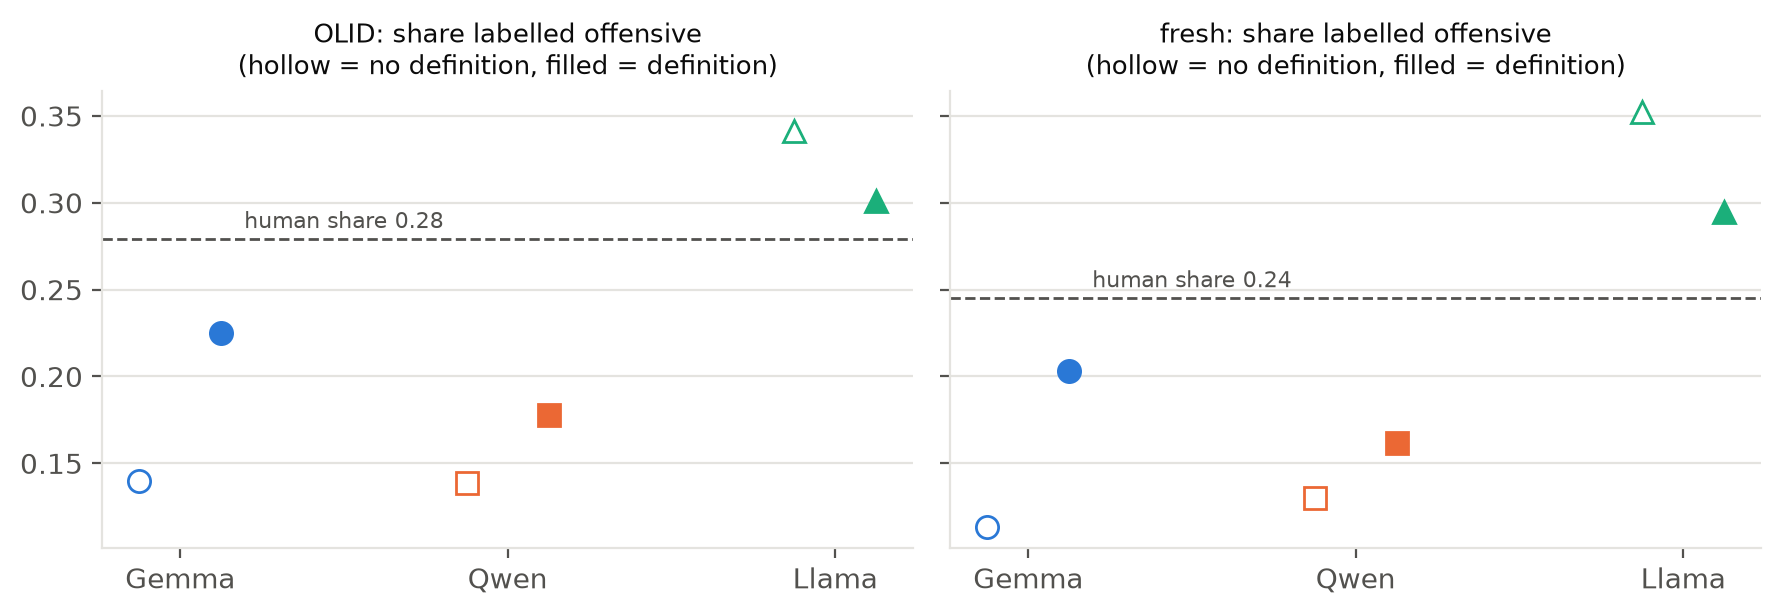
\includegraphics[width=0.82\textwidth]{figures/fig7_v3_prevalence_by_dataset.png}
  \caption{Share of posts labelled offensive, averaged over the three wordings, without (hollow) and with (filled) OLID's definition. Dashed line: human share.}
  \label{fig:prev}
\end{figure*}

\begin{table}[t]
  \centering\small
  \begin{tabular}{@{}>{\raggedright\arraybackslash}p{1.9cm}>{\raggedright\arraybackslash}p{2.45cm}>{\raggedright\arraybackslash}p{2.45cm}@{}}
    \toprule
    Probe & OLID test & New posts \\
    \midrule
    P1 guided & Llama $+0.022$ & Llama $+0.020$ \\
    P2 near-copies & \multicolumn{2}{>{\raggedright\arraybackslash}p{5.1cm}@{}}{6 completions overall, all famous quotes or stock phrases} \\
    P3 cue gain & $+0.005$ to $+0.020$ & $-0.009$ to $+0.031$ \\
    P4 Min-K\% & \multicolumn{2}{>{\raggedright\arraybackslash}p{5.1cm}@{}}{OLID test vs.\ new: Qwen 0.36, Llama 0.46; Gemma excluded (129/724 failures)} \\
    P5 quiz & 44--67\% & 53--70\% \\
    \bottomrule
  \end{tabular}
  \caption{Contamination battery (ranges over models; chance in P5 is 25\%). No probe shows OLID as more familiar than unseen posts.}
  \label{tab:contam}
\end{table}

\paragraph{Contamination.} No probe showed OLID as more familiar than the new posts (Table~\ref{tab:contam}; P1: ROUGE-L gain, P3: accuracy gain, P4: AUC, P5: accuracy). Two signals that would look like evidence on their own, Llama's guided-completion gain and quiz accuracy far above chance, are just as large on posts that cannot have been memorised. Following our pre-registered wording, the verdict is ``no evidence detected'', not evidence that OLID is absent from training data.

\paragraph{Exploratory and robustness results.} Posts whose label flipped across wordings had lower first-token confidence than stable posts for all models (e.g.\ Qwen $-0.27$ on the new posts). Between-model disagreement under W0 was much larger than wording disagreement: Llama disagreed with Gemma on 24.5\% and with Qwen on 23.0\% of new posts. The H1 and H3 conclusions were unchanged when invalid answers were counted as errors, OLID duplicates were removed, posts with annotator disagreement were removed, or OLID was matched on post length. With annotator A's labels alone, H3 remained significant for Gemma and Qwen but not for Llama ($\Delta_3 = -0.032$, $p_{\text{Holm}} = 0.91$; Appendix~\ref{app:sens}).

\section{Discussion}

Wording sensitivity did not disappear, or detectably grow, on posts the models cannot have seen. As far as our design can tell, the wording effects reported on benchmarks are not an artefact of memorised data, and they should be expected when LLMs label new material. They are, however, small compared with the other two choices a researcher makes. Including the definition shifted the estimated prevalence by up to nine percentage points, always toward the human share, which agrees with the view that annotation quality depends on how well the model's concept matches the task definition \citep{casanova2026limits,atreja2025prompt}. The choice of model changed roughly one label in four. For CSS practice this means that the definition belongs in the prompt and in the paper, several wordings should be tested, and model output should be validated against human labels \citep{pangakis2023automated}.

The contamination battery illustrates why negative controls matter. Without the new posts, Llama's completion gain and the quiz accuracy above chance could have been read as evidence of memorisation; with them, both turn out to be properties of the probes. This is consistent with the warnings of \citet{duan2024membership} and \citet{zhang-etal-2026-test}.

\section{Limitations}

That OLID is in the models' training data is an assumption: no probe detects it, so a null H1 may mean either that memorisation does not drive wording sensitivity or that OLID is not memorised strongly enough to matter. The two datasets also differ in platform, year and topic, so the contrast is not purely one of exposure, although matching on length did not change H1. H1 has limited power (roughly 35--40\% for a true difference of 0.01), so small differences cannot be ruled out. Three one-sentence wordings are a lower bound on realistic prompt variation. Our gold labels come from our team rather than OLID's annotators, which is why H2 cannot be interpreted, and Llama's H3 result depends on how disagreements were resolved. Finally, we rely on the maKI service to serve the published model weights, and Qwen~3.6's training cut-off is not published; our argument for Qwen rests on its release date.

\section*{Ethics Statement}

We used public Bluesky posts obtained through the platform's official API. No post text is published in the repository, the paper or the slides; examples are invented or shown as model answers only. Author identifiers are stored only as salted hashes, and the raw download is deleted after the course. Annotators were members of the research team.

\section*{Use of AI Tools}

Code, documentation and drafts of this report and the slides were written with the assistance of Claude (Anthropic) and reviewed and edited by the team, which is responsible for all content. No LLM produced any human label.

\section*{Acknowledgements}

% Confirm the required wording with the instructors before submission.
Model queries were run on the maKI service of the University of Mannheim.

\bibliography{references}
\IfFileExists{acl_natbib.bst}{\bibliographystyle{acl_natbib}}{\bibliographystyle{plainnat}}

\appendix

\section{Prompts}
\label{app:prompts}

All prompts share the ending \texttt{Post: "\{text\}"} followed by \texttt{Answer with exactly one label: OFFENSIVE or NOT\_OFFENSIVE.} The first sentence differs by wording:

\begin{itemize}
  \item W0, R0: \emph{Does the following social-media post contain offensive language?}
  \item W1: \emph{Determine whether offensive language is present in the following social-media post.}
  \item W2: \emph{Classify the following social-media post based on whether it contains offensive language.}
\end{itemize}

D0--D2 and RD0 insert, after the first sentence: \emph{Use these definitions: OFFENSIVE: Posts containing any form of non-acceptable language (profanity) or a targeted offense, which can be veiled or direct. NOT\_OFFENSIVE: Posts that do not contain offense or profanity.}

\section{Sensitivity Analyses}
\label{app:sens}

\begin{table}[h]
  \centering\small
  \begin{tabular}{p{3.7cm}cc}
    \toprule
    Analysis & H1 sig. & H3 sig. \\
    \midrule
    Main analysis & none & G, Q, L \\
    Invalid answers as errors & none & G, Q, L \\
    OLID duplicates removed & none & G, Q, L \\
    Annotator disagreement removed ($n = 365$) & none & G, Q, L \\
    OLID matched on length ($n = 239$) & none & G, Q, L \\
    Gold = annotator A only & none & G, Q \\
    \bottomrule
  \end{tabular}
  \caption{Models significant after Holm correction (G = Gemma, Q = Qwen, L = Llama). H2 is not interpretable in any analysis.}
\end{table}

\end{document}
